\section{System Design Goals and Overview}
    We start this section by defining the design goals of our authentication system. We then gives an system overview which leverages the dynamic deformation features of facial expressions to authenticate identity. 
    \begin{figure*}[!ht]
        \centering
        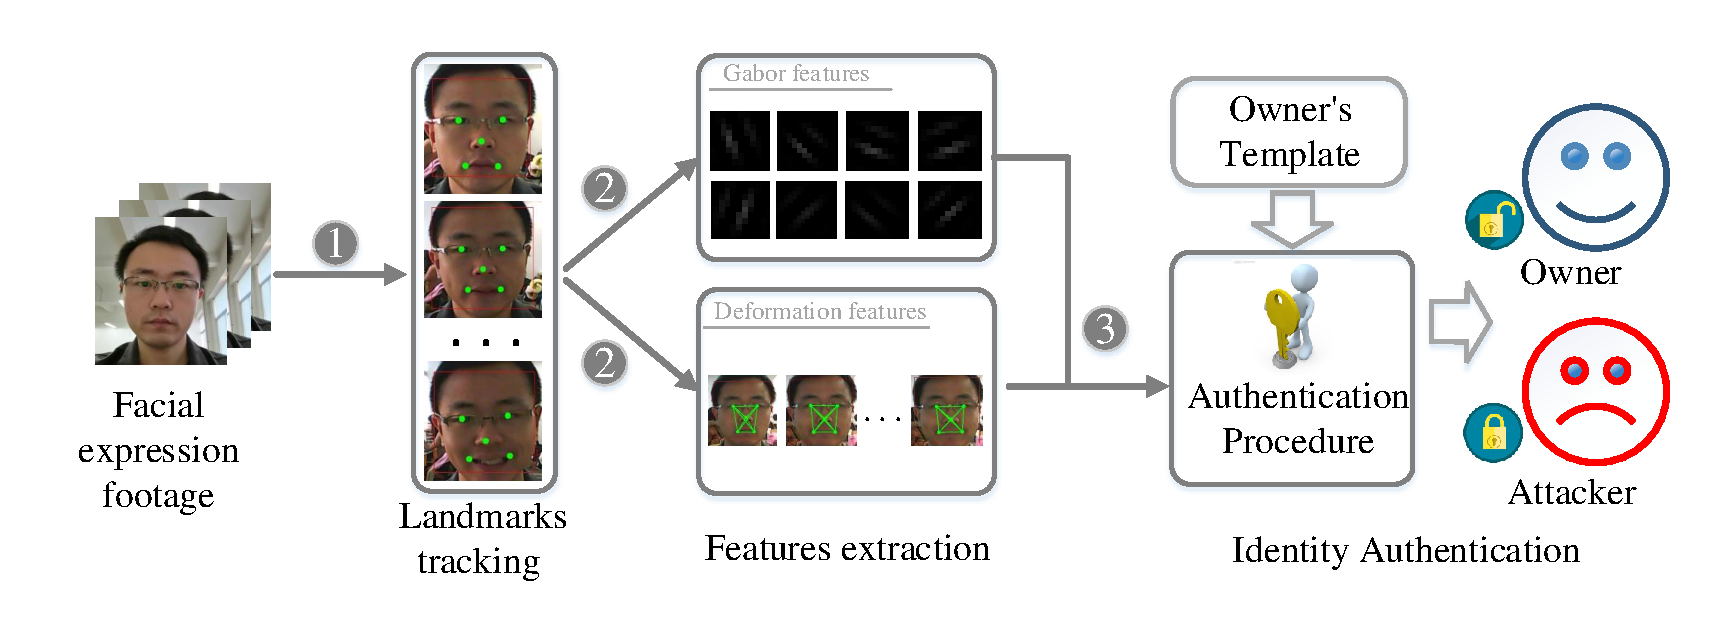
\includegraphics[width=\textwidth]{fig/overview.pdf}
        \caption{Overview of the attack.}
        \label{fig:overview}
    \end{figure*}
    \subsection{Design Goals}
        Biometrics which refers to either the static physiological traits or dynamic behavioral modalities are all non-revocable. This is one of the major reasons why biometrics is possible to be stolen or replayed by an expert adversary. Unlike traditional biometrics, facial behavioral traits is unique and can be changed with the changes of facial expressions. This is the biggest difference comparing with other biometric-based authentication systems. Therefore, facial behavior-based modalities are more secure than other biometrics in some extent.  Furthermore, it is possible to decrease the authentication time as much as possible with the development of facial detection technologies as well as not requiring the visual stimuli. This making facial biometrics are more user-friendly. In conclusion, a secure biometric-based authentication system should be secure, fast and user-friendly. The following we summary the design goals of our system:
        \begin{itemize}
            \item \emph{Simple:} This system should be simple as much as possible. Specifically, user should be minimal coordinate the system during authenticating process.
            \item \emph{Fast:} A single authentication duration should be as short as possible.
            \item \emph{Secure:} The system is able to immune to the replay and impersonation attacks.
            \item \emph{Revocable:} The biometrics can be changed once it is stolen or leakage.
        \end{itemize} 
    
    \subsection{System Overview}
        The system authenticates the user's identity by analyzing the dynamic changes of facial expressions. It records the entire change of facial expressions using in-built front camera of smartphone. The deformation features of facial expressions are extracted by existing facial detection algorithm and they are used to recognize the user's identity.
        Figure ~\ref{fig:overview} depicts the steps of this system:
         